The Results test the three propositions in sequence, moving from the qualification rule to
target-specific evidence and then to an integrated decision map. Each subsection therefore
states the question being tested before reporting its analysis frame, evidence, limitation,
and qualification decision.

\subsection{Qualification framework converts the propositions into evidence tests}

We begin by converting the study propositions into explicit evidence dimensions and decision
rules that will be applied consistently to every target.

\paragraph{Analysis frame.}
Candidate signals were evaluated at their fixed analysis unit whenever an endpoint was
available.
The Results follow the evidentiary sequence introduced above. We first test whether
morphology-linked signals transport across cohorts, then ask whether molecular and outcome
signals survive confounder, site, representation and endpoint audits, and finally integrate
those findings into target-specific evidence states. Each claim is linked to its cohort,
endpoint, frozen encoder output and saved source table (Figure~\ref{fig:qualification-framework}).

\paragraph{Evidence test.}
Five dimensions were kept distinct: cross-cohort transport, grade-adjusted increment, site
behavior, correlated setting sensitivity and endpoint dependence. They produced three
submission-facing states: transportable, context-sensitive and unsupported in the frozen
design. Support on one dimension did not substitute for missing evidence on another. The
complete target-by-axis coverage audit is provided in the supplementary evidence matrix and
its source-linked audit table.

\paragraph{Interpretive boundary.}
Not every target had a second cohort with the same label, and setting comparisons reused
patients and folds. The framework therefore qualifies the evidence available for each
target; it does not assume equal validation opportunities or convert statistical
non-support into biological absence.

\paragraph{Qualification rule.}
No pooled metric alone qualified a signal. A target's state was assigned only after the
relevant evidentiary axes had been considered together.
Figure~\ref{fig:qualification-framework} names the evaluated targets explicitly: PTEN denotes
phosphatase and tensin homolog loss, SPOP denotes speckle type BTB/POZ protein mutation, and
AR denotes androgen-receptor activity. Its two exploratory recurrence decisions concern a
post-hoc Cox risk score fitted in LEOPARD and transferred without refitting to TCGA-PRAD.
This score is called ``marker 7'' only in legacy analysis artifacts; it is referred to as the
post-hoc recurrence risk signal in the manuscript.

\paragraph{How to read the qualification map (Figure~\ref{fig:qualification-framework}).}
The horizontal position of each dot records an evidence decision, not an effect size or a
ranking. Grade and phenotype occupy the transportable column because their directions were
retained in cross-cohort evaluations without target-cohort refitting. PTEN remains
context-sensitive because its within-cohort signal did not establish a held-out increment
beyond grade and was not externally qualified. AR is also context-sensitive because its
positive pooled direction coexisted with unresolved site transport and no established
grade-independent increment. SPOP is unsupported in the frozen primary design because the
primary estimate did not separate from its null and the broader audit was
configuration-sensitive; this decision does not imply biological absence.

The two recurrence rows apply different questions to the same post-hoc Cox risk score.
Recurrence transfer asks whether the LEOPARD-fitted score retains prognostic association in
TCGA-PRAD without refitting, whereas recurrence increment asks whether that score adds
information beyond a clinical reference model. Both decisions remain exploratory and
context-sensitive because their interpretation changed with endpoint, covariate hierarchy,
or representation setting. Panel b counts how many decisions were primary or exploratory;
its bar lengths do not encode performance, effect magnitude, or evidentiary strength.

\begin{figure}[htbp]
\centering
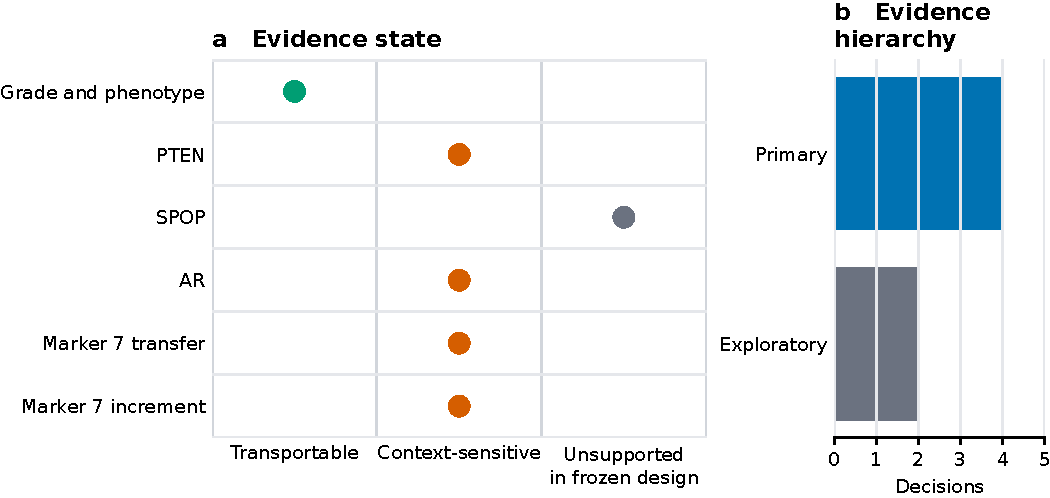
\includegraphics[width=\textwidth]{figures/fig1_qualification_map.pdf}
\caption{\figQualificationLegend}
\label{fig:qualification-framework}
\end{figure}

\subsection{Morphology-linked signals show the strongest cross-cohort transport}

Having defined the qualification rule, we first test whether grade and phenotype signals
retain their direction when applied to cohorts beyond the source data.

\paragraph{Analysis frame.}
The frozen NADT-Prostate CONCH probes were evaluated on patients in the source cohort and
then applied without refitting to PANDA case images from Karolinska and Radboud. PANDA used a
100-case cap per institution--International Society of Urological Pathology (ISUP) stratum:
1,200 sampled cases were drawn and 1,137 passed tissue filtering. The phenotype label
defined ISUP 0 as benign and ISUP $\geq1$ as tumor.
A separate PRECISE analysis used evaluable imaging sessions with pathologist-assigned Gleason
scores (Figure~\ref{fig:transportable-signals}).

\paragraph{Evidence state.}
Among 39 NADT-Prostate patients, the patient-level Gleason correlation was $0.478$
(95\% percentile patient-bootstrap interval $0.170$--$0.712$; 2,000 requested resamples;
valid and undefined replicate counts were not retained in the saved legacy output), and the
phenotype correlation was $0.800$ (95\% percentile patient-bootstrap interval
$0.625$--$0.909$; 2,000 requested resamples; valid and undefined replicate counts were not
retained in the saved legacy output). In PANDA, Gleason correlations were $0.354$ for 565 Karolinska cases
and $0.519$ for 572 Radboud cases; phenotype AUROCs were $0.786$ and $0.871$,
respectively, with 469/565 tumor cases at Karolinska and 483/572 tumor cases at Radboud. In PRECISE, the
session-level Gleason correlation was $0.865$ across 17 evaluable sessions. These consistent
cross-cohort directions supported a transportable state for grade and phenotype.

\paragraph{Local limitation.}
The saved source included no intervals for the PANDA and PRECISE rows. PANDA's capped sampling and
grade-derived phenotype label constrain interpretation of its case-image estimates, and
repeated encoder, scale and tile settings reused the same underlying cohorts.

\paragraph{Qualification decision.}
Grade signals retained a positive direction in both PANDA and PRECISE, whereas phenotype
discrimination was retained in the Karolinska and Radboud PANDA subsets. Together, these
results provided the strongest cross-cohort transport evidence among the evaluated targets.
However, no uncertainty intervals were saved for the PANDA or PRECISE estimates, limiting
conclusions about the precision of their effect sizes. This supports the first proposition
within the available cohorts, while remaining specific to these morphology-linked targets
and analysis units.

\begin{figure}[htbp]
\centering
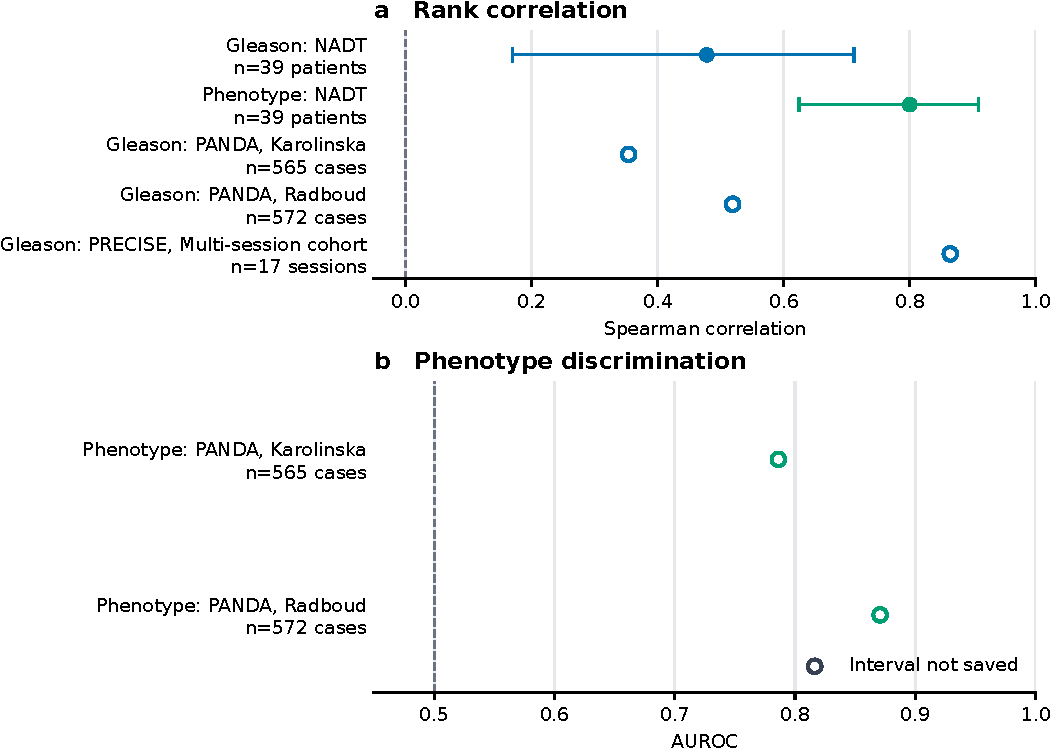
\includegraphics[width=\textwidth]{figures/fig2_transportable_signals.pdf}
\caption{\figTransportLegend}
\label{fig:transportable-signals}
\end{figure}

\subsection{Pooled molecular associations do not determine qualification}

We next ask whether pooled molecular associations are sufficient for qualification, or
whether the PTEN, AR, and SPOP signals require different evidentiary restrictions.

\paragraph{Analysis frame.}
PTEN loss, SPOP mutation and androgen-receptor (AR) activity were evaluated at the patient
level in the fixed 273-patient TCGA-PRAD frame using frozen CONCH outputs; the correlated
configuration summaries additionally included Virchow (Figure~\ref{fig:molecular-qualification}).

\paragraph{Evidence state.}
PTEN had a frozen-primary AUROC of $0.632$ (patient-bootstrap interval
$0.560$--$0.706$), and all evaluated cells were above chance, with a global seed-cell range
of $0.519$--$0.717$. AR had a frozen-primary Spearman correlation of $0.195$
($0.074$--$0.310$) and a global seed-cell range of $0.136$--$0.297$. SPOP had a
frozen-primary AUROC of $0.519$ ($0.408$--$0.627$), while its global seed-cell range crossed
chance ($0.348$--$0.679$). PTEN and AR were therefore context-sensitive; SPOP was
unsupported in the frozen primary design and configuration-sensitive in the broader audit.
The site-stratified SPOP audit did not overturn that decision (Figure~\ref{fig:molecular-qualification}c):
At the CH site (a deidentified source institution code), no patient was SPOP-positive and
the AUROC was therefore undefined, while
the saved patient-bootstrap interval at each of the other five source-coded sites included
the AUROC null.

\paragraph{Local limitation.}
PTEN and SPOP event counts were not recorded in the saved primary rows, and TCGA-PRAD did
not provide cross-cohort qualification for these molecular labels. The SPOP range neither
excludes a modest effect nor establishes biological absence.

\paragraph{Qualification decision.}
The pooled molecular results generated different questions rather than final claims: PTEN
required an increment audit, AR required site qualification, and SPOP remained unsupported
under the fixed primary design. This is the first test of the second proposition that a
positive or apparently stable pooled estimate can narrow under target-appropriate audits.

\begin{figure}[htbp]
\centering
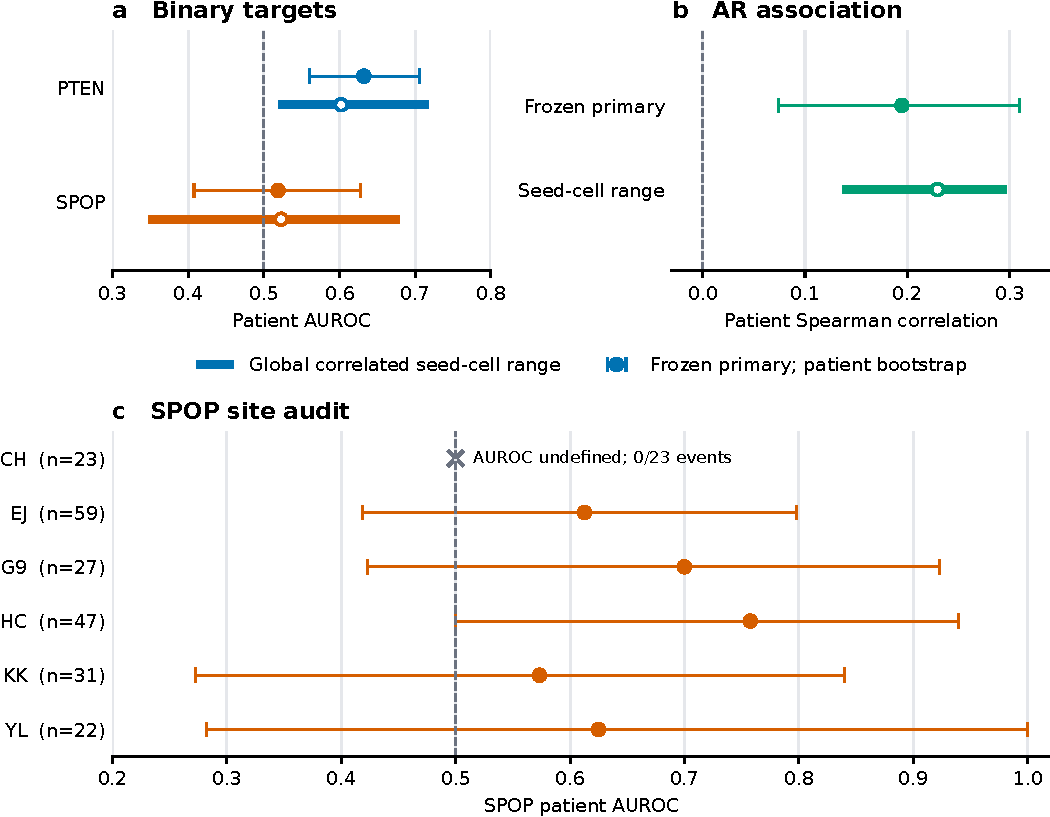
\includegraphics[width=\textwidth]{figures/fig3_molecular_qualification.pdf}
\caption{\figMolecularLegend}
\label{fig:molecular-qualification}
\end{figure}

\subsection{Confounder and site audits narrow the PTEN and AR claims}

Because pooled association alone cannot establish independent or transportable information,
this subsection tests whether the PTEN and AR signals persist beyond grade and across sites.

\paragraph{Analysis frame.}
Grade-adjusted increments were estimated on held-out TCGA-PRAD patients for CONCH and
Virchow. AR site analyses used slide-level correlations with patient-cluster bootstrap
intervals, whereas the pooled AR row used a patient-level estimate
(Figure~\ref{fig:confounder-site-audit}).

\paragraph{Evidence state.}
For PTEN, CONCH's held-out increment beyond grade was $+0.019$ (patient-bootstrap
interval $-0.025$ to $+0.068$); the Virchow increment was $+0.035$
($-0.013$ to $+0.087$). The corresponding AR increments in $R^2$ were $+0.004$
($-0.036$ to $+0.042$) and $+0.019$ ($-0.015$ to $+0.051$). The pooled AR correlation
was positive, but every stored site-specific interval crossed zero.

\paragraph{Local limitation.}
The site rows combine a slide-level effect estimate with patient-cluster resampling, and
site remains entangled with acquisition metadata. Binary endpoint event counts were not
available in the saved PTEN increment rows. No site or scanner cause can be assigned from
these comparisons.

\paragraph{Qualification decision.}
Grade-independent PTEN and AR increments were not established. AR's pooled direction was
supported, but site transport remained unresolved. The confounder and site audits therefore
narrowed the interpretation of the pooled signals, directly supporting the second
proposition.

\begin{figure}[htbp]
\centering
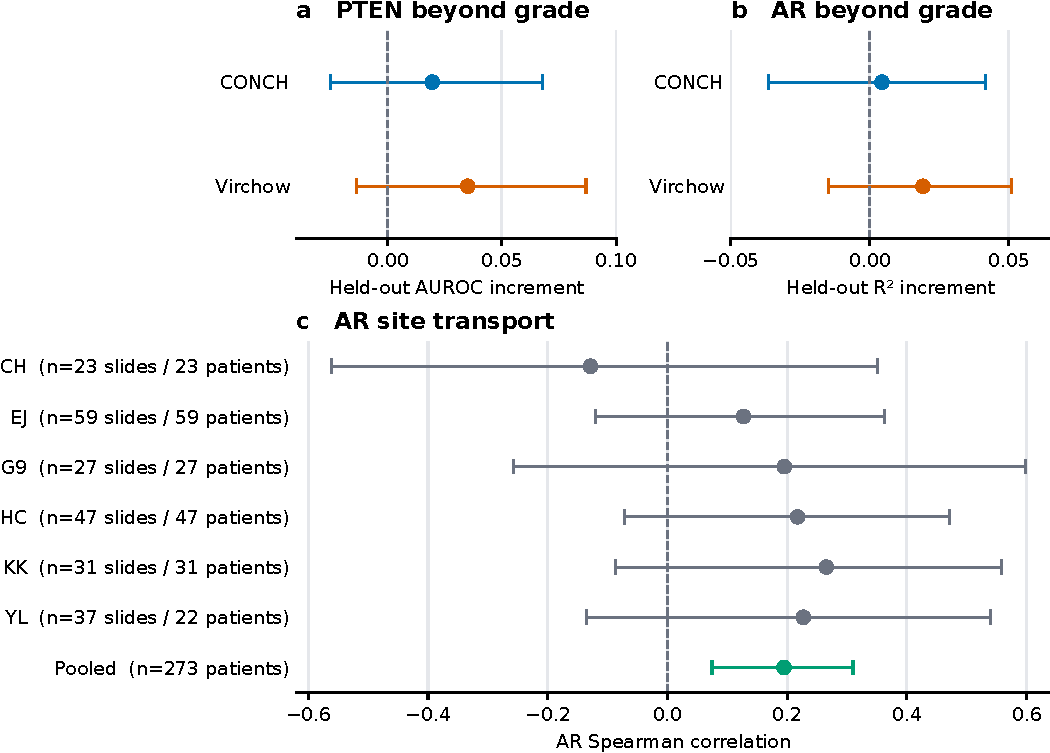
\includegraphics[width=\textwidth]{figures/fig4_confounder_site_audit.pdf}
\caption{\figConfounderLegend}
\label{fig:confounder-site-audit}
\end{figure}

\subsection{Recurrence transfer changes with endpoint and covariate hierarchy}

We then examine whether the exploratory recurrence signal retains the same interpretation
when the endpoint definition and the clinical reference model are changed.

\paragraph{Analysis frame.}
The post-hoc recurrence risk score was transferred from LEOPARD to a fixed 270-patient
TCGA-PRAD target frame. Frozen-risk performance was evaluated separately for the
Reconstructed with-tumor endpoint and the official TCGA Pan-Cancer Clinical Data Resource
progression-free interval (TCGA-CDR PFI). Increment analyses used the
same 153-patient complete-case cohort, with 30 reconstructed-endpoint events and 15 official
PFI events (Figure~\ref{fig:marker7-transfer}).

\paragraph{Evidence state.}
For the reconstructed endpoint, the concordance index (C-index) was $0.673$ (95\%
confidence interval (CI)
$0.587$--$0.759$; 270 patients, 57 events). The official PFI C-index was 0.586
(95\% CI 0.482--0.689; 270 patients, 42 events). The reconstructed endpoint
grade-plus-image versus grade delta C-index was $+0.083$ (95\% CI $+0.012$ to
$+0.157$), but its paired integrated Brier score (IBS) interval included zero. The official PFI
grade-plus-image increment was $+0.032$ ($-0.040$ to $+0.126$), and all official-PFI
paired C-index and IBS intervals include zero.

\paragraph{Local limitation.}
The recurrence risk signal was discovered post hoc, endpoint definitions differed, and multiple imputation
was not performed. The official-PFI result and every paired comparison were based on the
saved evaluable or complete-case frames; unobserved outcomes were not treated as events or
non-events.

\paragraph{Qualification decision.}
The recurrence signal remained exploratory and context-sensitive. Its effect and increment
depended on endpoint and covariate hierarchy, and the full clinical/site comparisons did
not support a general incremental claim. This provides an outcome-level demonstration of
the second proposition.

\begin{figure}[htbp]
\centering
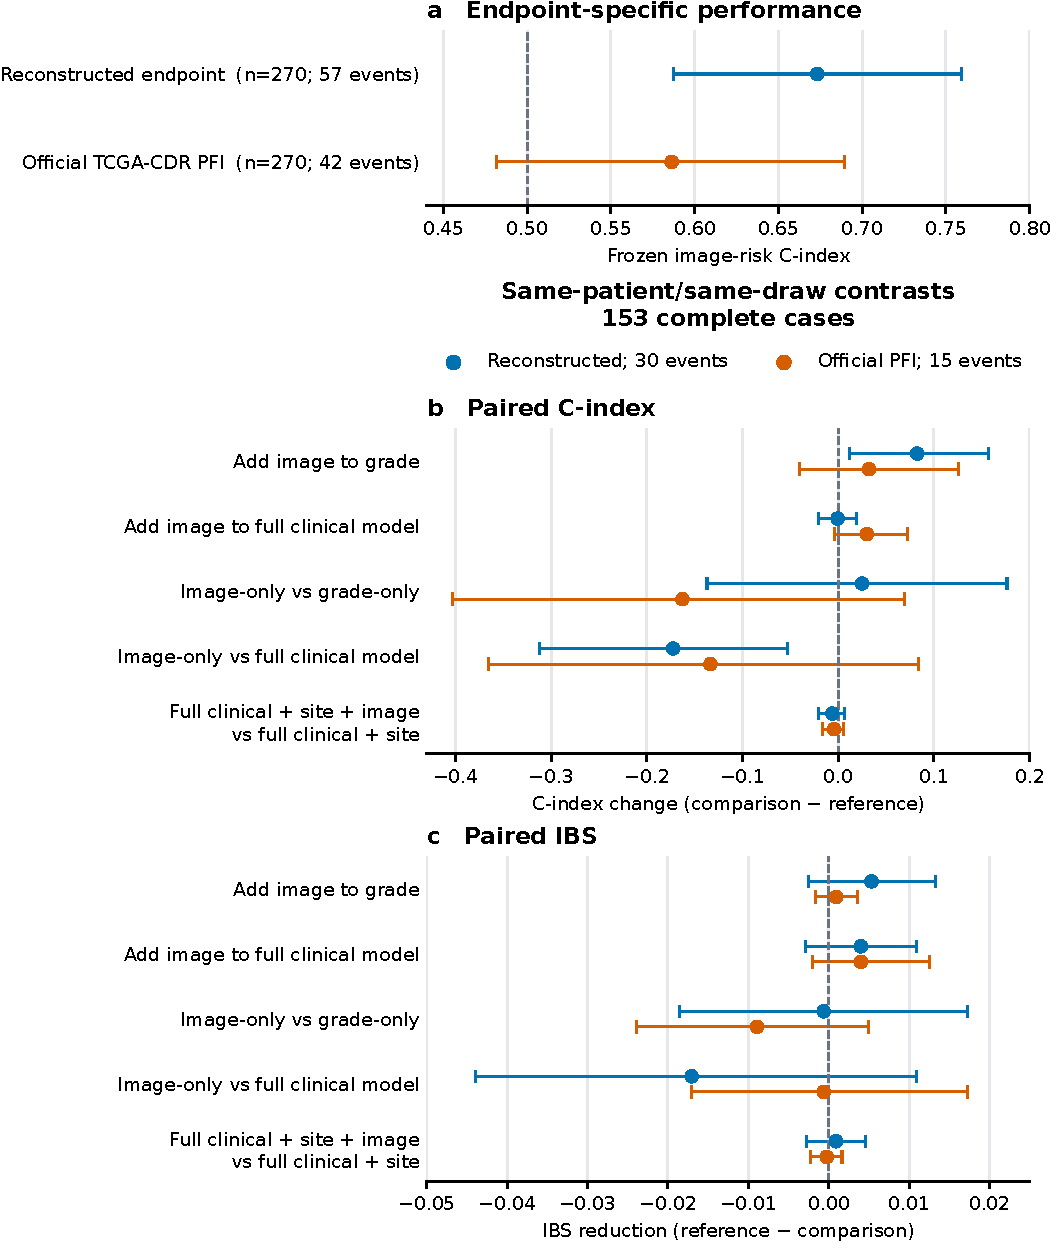
\includegraphics[width=\textwidth]{figures/fig5_marker7_transfer.pdf}
\caption{\figMarkerSevenLegend}
\label{fig:marker7-transfer}
\end{figure}

\subsection{Correlated setting audits distinguish stable from conditional signals}

After the cohort-, confounder-, site-, and endpoint-specific tests, we assess whether each
interpretation remains stable across the evaluated representation and sampling settings.

\paragraph{Analysis frame.}
Six targets were each summarized across 12 encoder--scale--tile configurations and five
sampling seeds, giving $6\times12\times5=360$ correlated seed cells. The post-hoc recurrence
risk signal's setting
sensitivity was interpreted alongside its endpoint-conditioned transfer summary
(Figure~\ref{fig:marker7-transfer}), and the decision-level grid summary is shown in
Figure~\ref{fig:stability-overview}. Paired
contrasts preserved shared patients, folds and settings.

\paragraph{Evidence state.}
No configuration's observed five-seed range straddled the metric null for Gleason,
phenotype, PTEN or AR. The observed five-seed range straddled the null for SPOP in $8/12$
configurations and the recurrence risk signal in $1/12$. Across the 60 seed cells for each
target, the global
seed-cell range was $0.271$--$0.646$ for Gleason and $0.845$--$0.965$ for phenotype; PTEN
remained above its null across all seed cells. SPOP and the recurrence risk signal showed greater setting
sensitivity than the transported signals.

\paragraph{Local limitation.}
The 360 cells are correlated sensitivity settings, not separate patient samples or repeated
confirmatory tests. A configuration's observed seed range and its descriptive Student-$t$
interval across seeds are different summaries; the $8/12$ and $1/12$ counts refer only to
observed-range straddling. Neither summary quantifies population uncertainty, and paired
contrast directions do not identify a causal effect of encoder, scale or tile budget.

\paragraph{Qualification decision.}
The stability audit bounded setting dependence without elevating evidence states. It
reinforced transported directions for grade and phenotype, preserved within-cohort PTEN
support, and narrowed SPOP and the recurrence risk signal to setting-conditioned
interpretations. Repeated
performance across correlated settings therefore informed robustness but did not constitute
independent validation.

\begin{figure}[htbp]
\centering
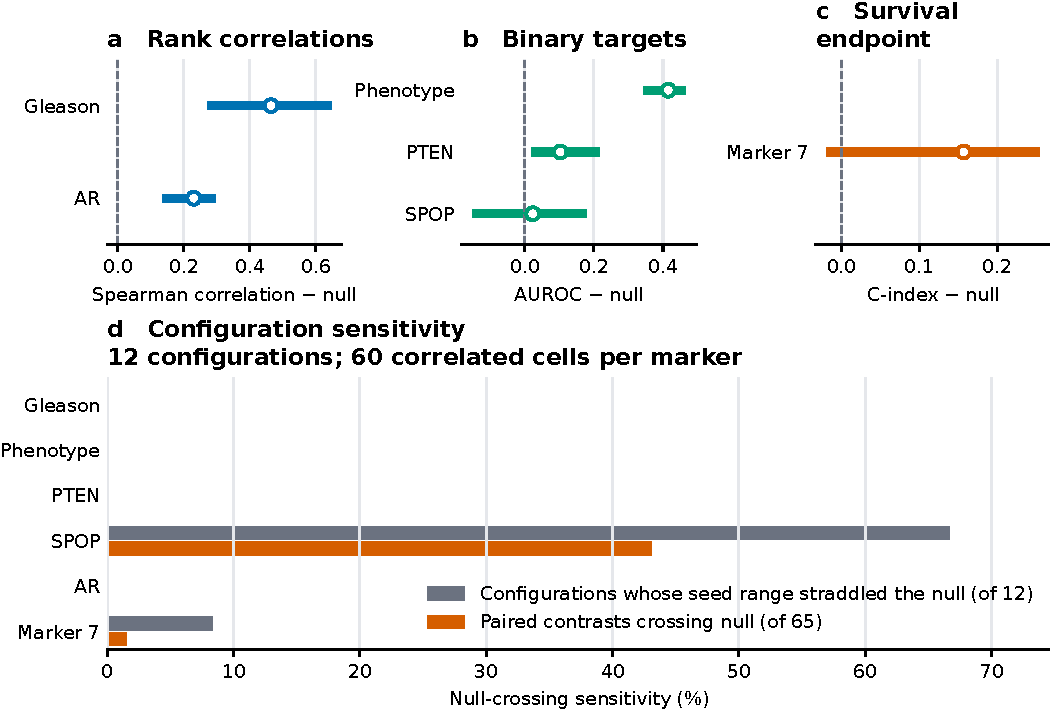
\includegraphics[width=\textwidth]{figures/fig6_stability_overview.pdf}
\caption{\figStabilityLegend}
\label{fig:stability-overview}
\end{figure}

\subsection{Joint evidence states replace a single performance ranking}

Finally, we integrate the preceding evidence axes to determine what can be claimed for each
target and what remains unresolved.

Across targets, the three propositions converged on one result: detectability and
qualification were not interchangeable. Morphology-linked grade and phenotype provided the
clearest transport evidence. Molecular signals separated after confounder and site audits,
and the recurrence signal changed with endpoint, covariate hierarchy and representation.
The correlated grid further showed that repetition across settings could either reinforce a
direction or expose conditionality, but could not replace external data.

The resulting evidence map (Table~\ref{tab:qualification-summary}) is the primary synthesis
of the study. It records the strongest support justified for each target together with the
axis that remains unresolved. Its purpose is not to rank encoders or biomarkers, but to
prevent a pooled association from being promoted beyond the evidence that qualifies it.

\paragraph{Qualification decision.}
The third proposition was supported: target-level evidence states conveyed distinctions
that a single performance ranking would conceal. These states remain research
qualifications, not claims of clinical validity or biological absence.

\begin{table}[htbp]
\centering
\small
\caption{Joint evidence map after target-specific qualification audits.}
\label{tab:qualification-summary}
\begin{tabular}{@{}p{0.18\textwidth}p{0.22\textwidth}p{0.52\textwidth}@{}}
\toprule
Evidence question & Evidence state & Supported interpretation \\
\midrule
Qualification logic & descriptive framework & marker-specific \\
Grade and phenotype transport & transportable & Externally transportable \\
PTEN qualification & context sensitive & Internally supported; multisite-stable \\
SPOP qualification & unsupported in frozen design & Primary unsupported; configuration-sensitive \\
AR qualification & context sensitive & Pooled direction supported; site transportability unresolved \\
Recurrence transfer & context sensitive & Post-hoc exploratory; endpoint/encoder/scale-limited \\
Recurrence increment & context sensitive & Exploratory; endpoint-conditioned \\
Setting sensitivity & descriptive framework & Descriptive sensitivity evidence \\
\bottomrule
\end{tabular}
\end{table}

